% *********************************************************************
% © 2016–2025 Jeremy Sylvestre
%
% Permission is granted to copy, distribute and/or modify this document
% under the terms of the GNU Free Documentation License, Version 1.3 or
% any later version published by the Free Software Foundation; with no
% Invariant Sections, no Front-Cover Texts, and no Back-Cover Texts. A
% copy of the license is included in the appendix entitled “GNU Free
% Documentation License” that appears in the output document of this
% PreTeXt source code. All trademarks™ are the registered® marks of
% their respective owners.
%
% *********************************************************************
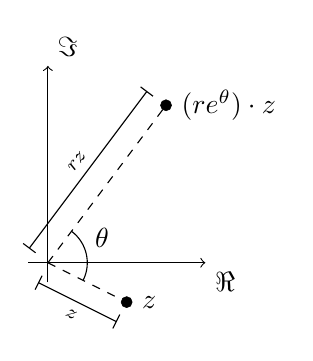
\begin{tikzpicture}[
	point/.style={circle,draw,very thin,fill,inner sep=0pt,minimum size=4pt},
]
	\draw[->] (-0.25,0) to (2,0) node[below right] {$\Re$};
	\draw[->] (0,-0.25) to (0,2.5) node[above right] {$\Im$};

	\node[point] at (1,-0.5) (z) [label=right:{$z$}] {};
	\node[point] at (1.5,2) (pz) [label=right:{$(r e^{\ci\theta}) \cdot z$}] {};

	\draw[dashed] (0,0) -- (z);  % slope is -1/2, perp slope is 2/1
	\draw[|-|,thin,yshift=-0.25cm,xshift=-0.125cm] (0,0) to node[below,sloped] {$\scriptstyle \cmodulus{z}$} (1,-0.5);
	\draw[dashed] (0,0) -- (pz);  % slope is 4/3, perp slope is -3/4
	\draw[|-|,thin,yshift=0.18cm,xshift=-0.24cm] (0,0) to node[above,sloped] {$\scriptstyle r \cmodulus{z}$} (1.5,2);

	\draw (0,0) ++(-26.565:0.5cm) arc (-26.565:53.13:0.5cm) node[midway,xshift=0.2cm,yshift=0.2cm] {$\theta$};


\end{tikzpicture}
